\chapter{Discussion}
\label{sec:discussion}

% Downbeat, Downbeat > Downbeat, Upbeat > Upbeat, Upbeat. Combination should use this hierarchy but doesn't really.
% However in combination with the top-down likelihood function it may.
% Expression
% Tempo curves are not relevant anymore. A subdivision approach may be a good way of researching expression in rhythm
% Cognitive plausibility
%	Incremental parsing
%	The bottom-up/top-down estimation of onset times doesn't seem to be very cognitively plausible.
% Other time signatures were not allowed, but theoretically it should be trivial to extend the present method for more time signatures.
% Swing ratio
% Does a pcfg captures temperleys common practice rhythm assumptions
% Combination/observations convoluted
% Not including rests leads to loss of information
% Parser produced interpretation that was very plausible given that tracks were played along an accompaniement some subtleties are lost when listening to the melody only


This chapter will discuss he effectiveness of the PCFG prior, the positive aspects of parsing subdivision trees. Finally a number of flaws in the model are discussed.

\section{Subdivision Parsing}

Our results show that subdivision parsing in general has been a successful approach. A completely tempo-independent parser was able to produce F-scores of around 0.8. Figure \ref{fig:a_fine_romance:a} and \ref{fig:a_fine_romance:b} illustrate how the parser interpreted the rhythmic structure of the onset pattern almost completely correct. By combining pitch information with the parser's analysis and setting a bar's duration to correspond to level 1/8 in the tree, we can generate a transcription of the onset pattern. This is illustrated in figure \ref{fig:a_fine_romance:c}.

To generate a score from a subdivision tree we need to set two variables by hand: the time signature and bar duration (in terms of level of the tree). The subdivision tree does specify whether beats are duple or triple divided, but it does not differentiate between 4/4, 2/2 and 2/4 for example. Deriving the correct time signature is not trivial and it may depend on how beats are stressed. However, this problem may be adequately addressed using a simple model that tries to find a tactus level in the tree, preferring intervals around 100ms. This is similar to the approach in  \citet{temperley2009unified, temperley2007music}, the difference being that in those models finding the tactus level is the first step in constructing the rhythmic structure while we first construct the rhythmic structure and then find the tactus level to get the correct time signature.

As mentioned earlier, the parser's interpretation in figure \ref{fig:a_fine_romance:c} differed slightly from the gold-standard gold standard in figure \ref{fig:a_fine_romance:c}. The difference is lies in the way the parser interpreted the first onset. The gold standard specifies that the first bar should be divided into two half notes, the first half note is divided in two quarter notes and the rightmost of these quarter notes is divided into an eighth note triplet with an onset on the last position. Instead of this rather complicated analysis, the parser simply divided the bar in a half note triplet with an onset on the last position. 

Further inspection of the two interpretations reveals that they are interchangeable. Triple divisions introduce an ambiguity in subdivision trees, illustrated in figure \ref{fig:ambiguity}. The parser chose the simplest interpretation since it has the highest prior probability. The difference between the two analyses can be expressed as a difference in time signature. The analysis on the left in figure \ref{fig:ambiguity} implies a 3/2 time signature, the analysis on the right implies a 4/4 time signature where the third beat is divided into three eighth notes.

The gold-standard in figure \ref{fig:a_fine_romance:d} was chosen because we assume the time signature not to change unless the performance gives us clear evidence that it should change. There is a certain consistency of time signature. The rhythm model as it was presented here has does not penalise changes in time signature and adding this could be a potential improvement to the model.


\begin{figure}
\centering
\subfloat[The raw onset times of the performance (in seconds).]{
\label{fig:a_fine_romance:a}
[2.62, 3.03, 4.52, 4.92, 5.65, 6.02, 7.54, 7.91, 8.53, 9.04, 10.51, 10.89, 11.53, 12.05]
}

\subfloat[The interpretation generated by the parser.]{
\label{fig:a_fine_romance:b}
\Tree
[ .{$\frac{1}{1}$} [ .{$\frac{1}{2}$} [ .{$\frac{1}{4}$} [ .{$\frac{1}{8}$} [ .$*$ ] [ .$*$ ] [ .$\bullet$ ] ] [ .$\bullet$ ] ] [ .{$\frac{1}{4}$} [ .{$\frac{1}{8}$} [ .{$\frac{1}{16}$} [ .$\bullet$ ] [ .$\bullet$ ] ] [ .{$\frac{1}{16}$} [ .$*$ ] [ .$\bullet$ ] ] ] [ .$\bullet$ ] ] ] [ .{$\frac{1}{2}$} [ .{$\frac{1}{4}$} [ .{$\frac{1}{8}$} [ .{$\frac{1}{16}$} [ .$\bullet$ ] [ .$\bullet$ ] ] [ .{$\frac{1}{16}$} [ .{$\frac{1}{32}$} [ .$*$ ] [ .$*$ ] [ .$\bullet$ ] ] [ .$*$ ] ] ] [ .$\bullet$ ] ] [ .{$\frac{1}{4}$} [ .{$\frac{1}{8}$} [ .{$\frac{1}{16}$} [ .$\bullet$ ] [ .$\bullet$ ] ] [ .{$\frac{1}{16}$} [ .{$\frac{1}{32}$} [ .$*$ ] [ .$*$ ] [ .$\bullet$ ] ] [ .$*$ ] ] ] [ .$\bullet$ ] ] ] ]
}

\subfloat[A score generated from the subdivision tree combined with pitch information. The bar duration was set to correspond to the 1/4 level in the tree.]{
\label{fig:a_fine_romance:c}
\includegraphics[width=\textwidth]{img/a_fine_romance}
}

\subfloat[The gold-standard score.]{
\label{fig:a_fine_romance:d}
\includegraphics[width=\textwidth]{img/a_fine_romance_gs}
}
\caption{A interpretation that was completely identical to the gold standard.}
\label{fig:a_fine_romance}
\end{figure}

\begin{figure}
\Tree
[ .{$\frac{1}{1}$} [ .$*$ ] [ .$*$ ] [ .$\bullet$ ] ] 
\Tree
[ .{$\frac{1}{1}$} [ .$*$ ] [ .{$\frac{1}{2}$} [ .{$\frac{1}{4}$} [ .$*$ ] [ .$*$ ] [ .$\bullet$ ] ] [ .$*$ ] ] ]

\caption{An ambiguity introduced by triple divisions.}
\label{fig:ambiguity}
\end{figure}

\section{The Rhythm Model}

%The example in figure \ref{fig:a_fine_romance} shows that the rhythm model successfully prevents analyses that are to complicated. The phase 

%As can be seen in table \ref{tab:rhythm}, given the constraints that we imposed on subdivision, the model has a limited number of parameters. % Picture of phase shifting a rhythm and its probabilities.

A more thorough evaluation of our rhythm model would be to compare its performance to Temperley's hierarchical model, used in \citep{temperley2009unified}. We could for example exchange our prior for Temperley's and compare the parser's  performance on our corpus. We did not implement this comparison at present for two reasons: First, Temperley did not, as far as we know, specify how his hierarchical model generalises to triple divisions. Second, the hierarchical model is defined relative to the levels of a metrical grid. Levels in our model do not correspond trivially to levels in a metrical grid. 

\section{The Expression Model}

It could not be shown in this study that simple rhythmic expression can help analysing rhythms. However, it may be that our model simply is not adequate for this purpose. In this section the model will be discussed and some issues of the model will be linked to the low evaluation scores.

A high amount of noise level-one triple divisions seems to be the biggest contribution to the low evaluation scores. The high value of the $\sigma$ parameter for level-one triple divisons, combined with a prior that assigns a high probability to the rule $R \rightarrow \bullet\; *\; \bullet$, divisions like in figure \ref{fig:discuss1:a} are likely to be classified as the division in figure \ref{fig:discuss1:b}. Because of the high $\sigma$ for triple divisions at level one, the incorrect analysis in \ref{fig:discuss1:b} is not penalised very much and the high prior probability of analysis in figure \ref{fig:discuss1:b} may make the parser prefer it to the analysis in figure \ref{fig:discuss1:a}. The additive noise expression model sets $\sigma$ to be 0.1 for all levels and divisions and penalises the interpretation \ref{fig:discuss1:b} of \ref{fig:discuss1:a} more severely.

\begin{figure}
\centering
\subfloat[]{
\label{fig:discuss1:a}
\parbox{0.25\linewidth}{
\Tree
[ .{$\frac{1}{1}$} [ .$\bullet$ ] [ .$\bullet$ ] ]
}
}
\subfloat[]{
\label{fig:discuss1:b}
\parbox{0.25\linewidth}{
\Tree
[ .{$\frac{1}{1}$} [ .$\bullet$ ] [ .$*$ ] [ .$\bullet$ ] ]
}
}
\caption{Two competing interpretations of two onsets.}
\label{fig:discuss1}
\end{figure}

This interpretation is supported by some of the parses that the parser produced where duple divisions are interpreted as triple divisions. Figure \ref{fig:blue_bossa} shows the parser's interpretation of the first four measures of Kenny Dorham's Blue Bossa. The parser's interpretation is sometimes quite at odds with the gold standard, but given that the incorrectly interpreted divisions are all triple divisions at the lowest level, this parse is not penalised much for it.

\begin{figure}
\centering
\subfloat[Parser interpretation]{
\Tree
[ .{$\frac{1}{1}$} [ .{$\frac{1}{2}$} [ .{$\frac{1}{4}$} [ .$*$ ] [ .$*$ ] [ .$\bullet$ ] ] [ .{$\frac{1}{4}$} [ .{$\frac{1}{8}$} [ .$\bullet$ ] [ .$*$ ] [ .$\bullet$ ] ] [ .{$\frac{1}{8}$} [ .$\bullet$ ] [ .$\bullet$ ] [ .$\bullet$ ] ] ] ] [ .{$\frac{1}{2}$} [ .{$\frac{1}{4}$} [ .$*$ ] [ .$*$ ] [ .$\bullet$ ] ] [ .{$\frac{1}{4}$} [ .$\bullet$ ] [ .{$\frac{1}{8}$} [ .$\bullet$ ] [ .$*$ ] [ .$\bullet$ ] ] ] ] ]
}

\subfloat[Gold-standard]{
\Tree
[ .{$\frac{1}{1}$} [ .{$\frac{1}{2}$} [ .{$\frac{1}{4}$} [ .$*$ ] [ .{$\frac{1}{8}$} [ .$*$ ] [ .$\bullet$ ] ] ] [ .{$\frac{1}{4}$} [ .{$\frac{1}{8}$} [ .$\bullet$ ] [ .{$\frac{1}{16}$} [ .$*$ ] [ .$\bullet$ ] ] ] [ .{$\frac{1}{8}$} [ .{$\frac{1}{16}$} [ .$\bullet$ ] [ .$*$ ] [ .$\bullet$ ] ] [ .{$\frac{1}{16}$} [ .$*$ ] [ .$*$ ] [ .$\bullet$ ] ] ] ] ] [ .{$\frac{1}{2}$} [ .{$\frac{1}{4}$} [ .$*$ ] [ .{$\frac{1}{8}$} [ .$*$ ] [ .$\bullet$ ] ] ] [ .{$\frac{1}{4}$} [ .$\bullet$ ] [ .{$\frac{1}{8}$} [ .$\bullet$ ] [ .{$\frac{1}{16}$} [ .$*$ ] [ .$*$ ] [ .$\bullet$ ] ] ] ] ] ]
}
\caption{The parser interpretation and gold-standard of the first four measures of Kenny Dorham's Blue Bossa.}
\label{fig:blue_bossa}
\end{figure}

The down-/upbeat for divisions higher than two is calculated by averaging the beat lengths before the onset and dividing it by the average beat length after the onset (see equation \ref{eq:expression}). We do not use a feature for different kind of triple divisions but average all triple divisions together during training. One drawback of this approach is that the swing ratio is lost.

The question remains why the expression model is so noisy for triple divisions. It seems that the $\sigma$ parameter of roughly 0.7 cannot be caused only by variation in swing ratios. The exponential of 0.7 is approximately a ratio of 2, which seems unlikely to happen very often when performers are reasonably competent. After analysing the corpus, it was found that out of all 959 expression ratios at a level-one triple division, 81 had an expression ratio of higher than $\log(2)$ or lower than $\log(0.5)$. A few of those may have been caused by annotation errors but it seems that most of these are caused by the way the ratios are observed by the \textsc{observations} function.

The \textsc{observations} function however, partially relies on expected onsets calculated by the combination functions. This process is convoluted and makes it hard to track down what causes the outlier expression ratios.

It should also be noted that the level feature has an imperfection. In section \ref{sec:observations}, the \texttt{level} feature was defined as the depth of the hypothesis at which a expression ratio is observed. However the lowest level of a tree is not always the same level. Level one for example can be the quarter note level at some point in a performance and the eighth note level at another point in the same performance. 


\section{The Jazz Corpus}

Sometimes the parser produces interpretations that may have been more sensible to the listener than the gold-standard interpretation of a rhythm. An example of this is shown in figure \ref{fig:brazil}, which shows the rhythm of the first four measures of Chick Corea's Brazil. The gold-standard analysis claims that the first two beats are swung eighth-note upbeats. This is a very odd way for a piece to start. The parser makes the much more sensible suggestion that the second onset is actually a downbeat on the first beat of the second measure. The second onset is only a third of a quarter note away from the downbeat of the second measure so the parser's analysis is not very far off. 

\begin{figure}
\centering
\subfloat[Interpretation produced by the parser with the additive noise expression model.]{
\parbox{\linewidth}{
\Tree
[ .{$\frac{1}{1}$} [ .{$\frac{1}{2}$} [ .{$\frac{1}{4}$} [ .$*$ ] [ .$*$ ] [ .$\bullet$ ] ] [ .$\bullet$ ] ] [ .{$\frac{1}{2}$} [ .$*$ ] [ .{$\frac{1}{4}$} [ .{$\frac{1}{8}$} [ .$*$ ] [ .$\bullet$ ] ] [ .{$\frac{1}{8}$} [ .$\bullet$ ] [ .$\bullet$ ] ] ] ] ]
}
}

\subfloat[Gold-standard.]{
\parbox{\linewidth}{
\Tree
[ .{$\frac{1}{1}$} [ .{$\frac{1}{2}$} [ .{$\frac{1}{4}$} [ .$*$ ] [ .{$\frac{1}{8}$} [ .{$\frac{1}{16}$} [ .$*$ ] [ .$*$ ] [ .$\bullet$ ] ] [ .{$\frac{1}{16}$} [ .$*$ ] [ .$*$ ] [ .$\bullet$ ] ] ] ] [ .$*$ ] ] [ .{$\frac{1}{2}$} [ .$*$ ] [ .{$\frac{1}{4}$} [ .{$\frac{1}{8}$} [ .$*$ ] [ .$\bullet$ ] ] [ .{$\frac{1}{8}$} [ .$\bullet$ ] [ .$\bullet$ ] ] ] ] ]
}
}
\caption{A comparison of the parser and gold-standard interpretation of the first four measures of Chick Corea's Brazil.}
\label{fig:brazil}
\end{figure}


The reason why this performance oddly starts with two upbeats followed by a measure of silence is probably that it originally was accompanied by other instruments, in which case it would not be as unusual to start a melody like this. Since we are considering the melodies in isolation, we occasionally get melodies where it is, even to human listeners, not immediately clear where the downbeats are. The way the parser annotated this rhythm may well be the way that most listeners would interpret it. In any case, this seems to be a drawback of having a monophonic jazz corpus constructed from polyphonic MIDI files.




\section{Rests}

It was assumed early on that we could completely represent the rhythmic structure by looking only at onset times. It the evaluation section we referred to this section when we needed rests in the parse tree to represent a quarter note at the end of the performance. It turns out that, while we can completely specify the rhythmic structure for the most part using just onsets, we need rests to represent a performance that does not end on the last beat of a bar. Consider the gold-standard in in figure \ref{fig:rests:a} and a potential parser interpretation in figure \ref{fig:rests:b}. Figure \ref{fig:rests:b} implies that the last note, which is a quarter note in the gold standard, is a whole note like transcription A adjecent to it. Another interpretation is that the last note is a half note and the others eighth notes. Both of these interpretations are quite unlikely. In the current approach however, figure \ref{fig:rests:b} is not very unlikely as the parser considers only the onset of the last note and has no way of knowing how long the duration of the note is. And even if it would know the duration of the note, then given the current grammar, it would have no way of representing the last note as a quarter note. 

The only solution is to extend our approach to include rests. To do so would not require a great deal of changes. We can use roughly the same approach and add a \textit{rest} unit to the grammar, whose onset can be considered to be the offset of the previous note, tie or rest. In such an approach, rests would simply be another unit that have an onset which can be compared to its expected onset.

\begin{figure}
\centering
\subfloat[Gold-standard.]{
\label{fig:rests:a}
\parbox{0.5\linewidth}{
\Tree
[ .{$\frac{1}{1}$} [ .{$\frac{1}{2}$} [ .$\bullet$ ] [ .$\bullet$ ] ] [ .{$\frac{1}{2}$} [ .$\bullet$ ] [ .$\bullet$ ] ] ]
}
}
\subfloat[]{
\parbox{0.5\linewidth}{
\begin{tabular}{| l  >{\centering\arraybackslash}m{2in} |}
\hline 
A & 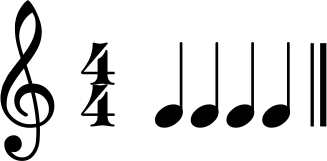
\includegraphics[scale=0.3]{img/discuss1}\\
\hline
\end{tabular}
}
}

\subfloat[Parser interpretation.]{
\label{fig:rests:b}
\parbox{0.5\linewidth}{
\Tree
[ .{$\frac{1}{1}$} [ .{$\frac{1}{2}$} [ .{$\frac{1}{4}$} [ .$*$ ] [ .$\bullet$ ] ] [ .{$\frac{1}{4}$} [ .$\bullet$ ] [ .$\bullet$ ] ] ] [ .$\bullet$ ] ] 
}
}
\subfloat[]{
\parbox{0.5\linewidth}{
\begin{tabular}{| l  >{\centering\arraybackslash}m{2in} |}
\hline 
A & 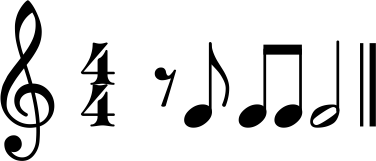
\includegraphics[scale=0.3]{img/discuss2}\\
B & 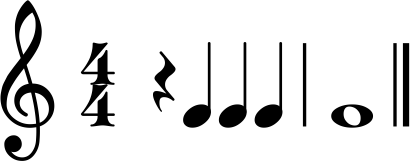
\includegraphics[scale=0.3]{img/discuss3}\\
\hline
\end{tabular}
}
}

\parbox{0.4\linewidth}{
\subfloat[A representation that includes rests.]{
\label{fig:rests:c}
\Tree
[ .{$\frac{1}{1}$} [ .{$\frac{1}{2}$} [ .{$\frac{1}{4}$} [ .$*$ ] [ .$\bullet$ ] ] [ .{$\frac{1}{4}$} [ .$\bullet$ ] [ .$\bullet$ ] ] ] [ .{$\frac{1}{2}$} [ .{$\frac{1}{4}$} [ .$\bullet$ ] [ .Rest ] ] [ .Rest ] ] ]
}
}
\subfloat[]{
\parbox{0.5\linewidth}{
\begin{tabular}{| l  >{\centering\arraybackslash}m{2in} |}
\hline 
A & 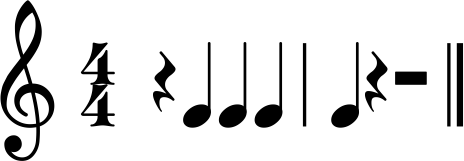
\includegraphics[scale=0.3]{img/discuss4}\\
\hline
\end{tabular}
}
}
\caption{An example of why rests are desirable to correctly represent the last note.}
\label{fig:rests}
\end{figure}
